\section{Ejercicio 8}

\par El scheduler SchedRR2 es una variación del tipo de scheduler Round-Robin que no permite migración de procesos entre nucleos. Para determinar en qué nucleo correrá un proceso se tienen en cuenta la cantidad de procesos activos totales de cada nucleo (blocked + running + ready) y se elije el que tenga la cantidad menor.

\par La característica de no permitir migración de procesos entre nucleos afecta el rendimiento notablemente con respecto a un scheduler que si lo permita: en algunos casos lo beneficia y en otros lo perjudica. A continuación vamos a analizar un caso para el cual el scheduler sale beneficiado y otro para el que no. \\\\

\textbf{Caso beneficioso}
\\
\par Un caso en el que el scheduler saldría beneficiado al no permitir la migración de procesos entre nucleos creemos que es un servidor que constantemente recibe peticiones (entre un grupo acotado). Al llegar una petición, se inicia un proceso que responda a ella. Estos procesos van a ir distribuyéndose entre los distintos nucleos. Al ser estos procesos de similar tamaño no va a ser necesaria la migración entre nucleos, ya que es dificil que se acumulen varios procesos en un nucleo y que el resto de los nucleos se liberen. Además, en caso de que esto ocurra lo mas probable es que a los procesos les quede poco tiempo de ejecución y hacer un cambio de nucleo (con los costos que esto genera) será mas perjudicial que beneficioso.
\par Creemos que para este caso el throughput va a ser un valor alto, ya que constantemente se inician procesos (para responder las peticiones) de tamaño similar, lo que implica que terminarán en un tiempo similar, dando como resultado constantes finalizaciones de procesos. El turnaround depende del promedio de la cantidad de procesos que lleguen, pero en general creemos que va a ser un tiempo bajo. El waiting time también depende de la cantidad de procesos que vayan llegando, pero al ser en su esencia un Round-Robin el proceso va a ser ejecutado cada poco tiempo. El tiempo de respuesta va a ser casi inmediato, el proceso sólo debe esperar que finalize la ronda de Round-Robin del nucleo al que fué asignado. Creemos que va a haber justicia (Fairness) en cuanto a la distribución de la CPU a los procesos por el solo hecho de que se trata de un Round-Robin, y el CPU se distribuyen de a quantums iguales. \\
\par Veamos un ejemplo de este caso. Creamos un lote de prueba con muchos procesos de similar tamaño que llegan cada tiempos reducidos y vamos a correr el scheduler para ver como se comporta.\\

\begin{figure}[h]
  \centering
    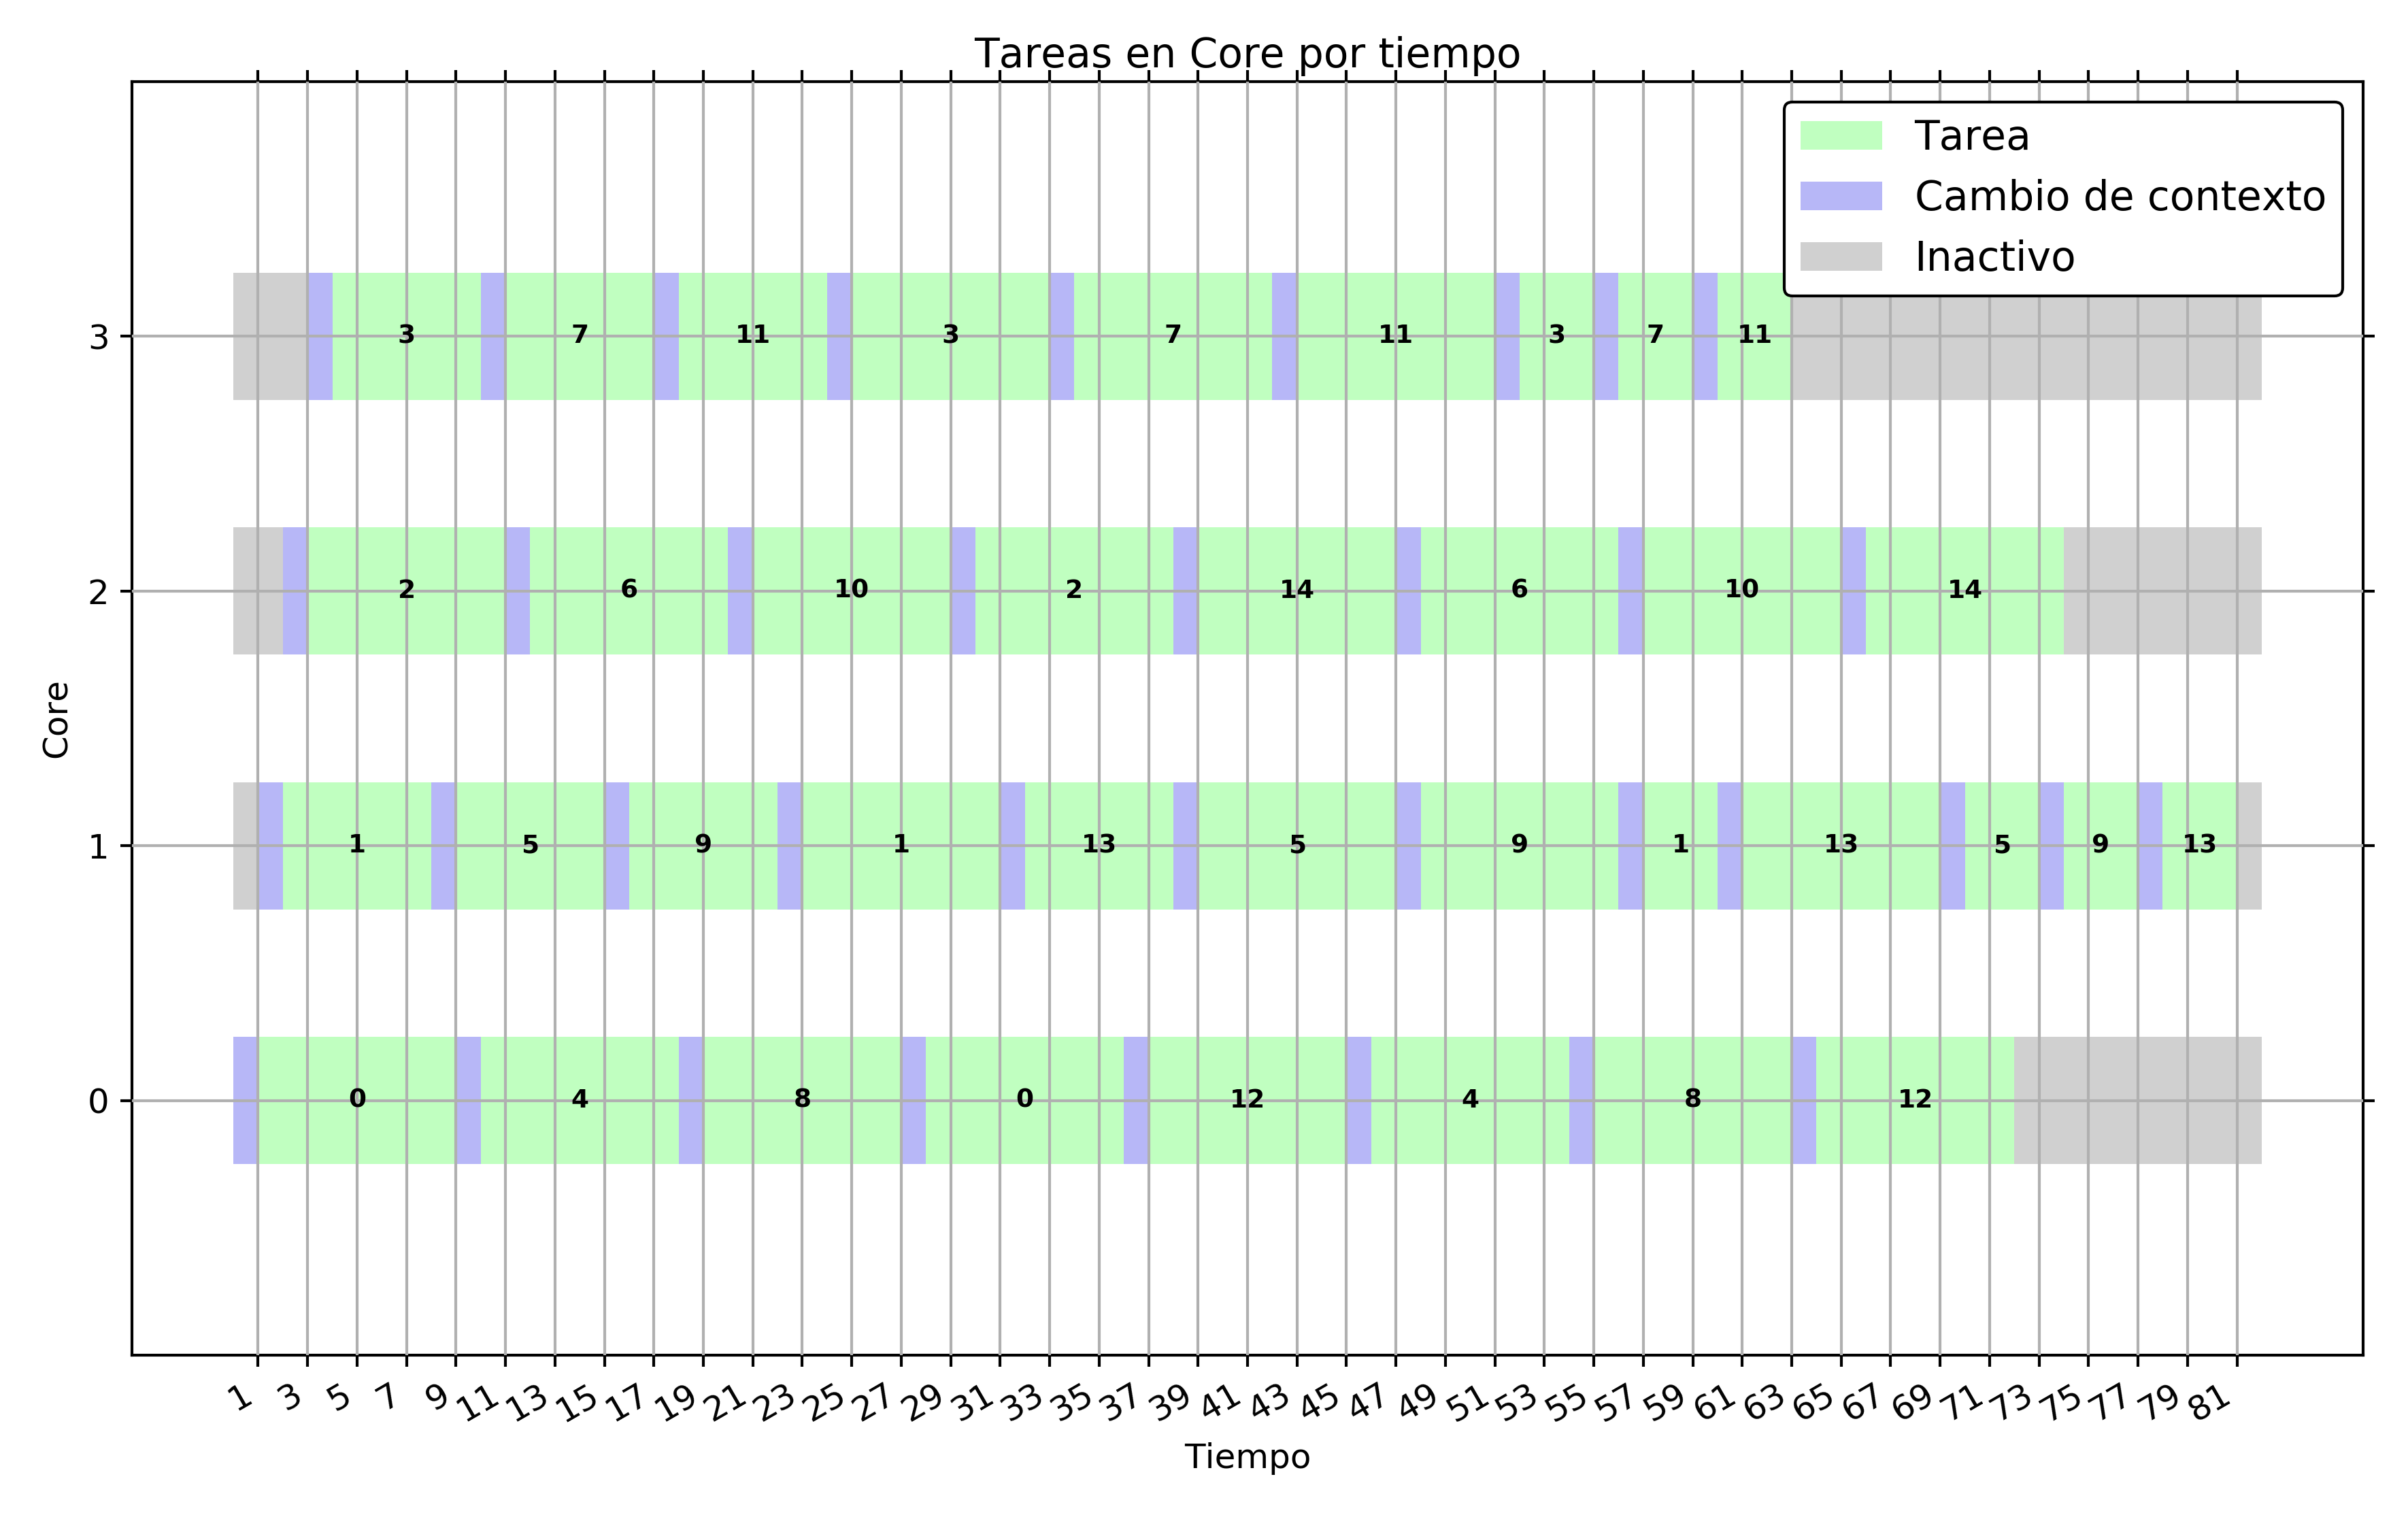
\includegraphics[width=1\textwidth]{images/ej8/lote1_cores.png}
  \label{fig: lote8_1_cores}
  \caption{Diagrama de uso de nucleos del lote 1.}
\end{figure}

\par En la figura \ref{fig: lote8_1_cores} podemos ver que los nucleos se mantuvieron ocupados de forma similar (casi sin momentos inactivos) y se liberaron en tiempos cercanos.

\begin{figure}[h]
  \centering
    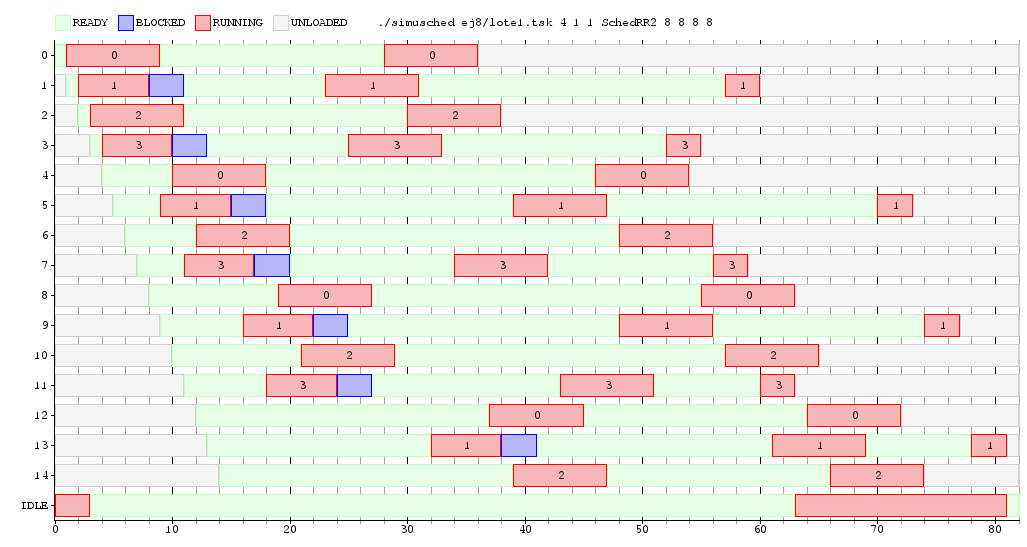
\includegraphics[width=1\textwidth]{images/ej8/lote1_sched.png}
  \label{fig: lote8_1_sched}
  \caption{Diagrama de procesos del lote 1.}
\end{figure}

\par En la figura \ref{fig: lote8_1_sched} podemos ver los distintos procesos y sus estados a lo largo de su tiempo de vida. Vemos que el lote cuenta con procesos similares y terminan con un formato similar al de la entrada (en escalera).\\\\
\par Analicemos el rendimiento del scheduler:
\begin{itemize}
	\item \textbf{Fairness:}
	\begin{itemize}
		\item 8 procesos reciben 2 quantums.
		\item 7 procesos reciben 3 quantums.
	\end{itemize}
	Como vemos los quantums se distribuyen de forma bastante justa entre los procesos.
	\item \textbf{Tiempo de respuesta:}\\
	Promedio: $\frac{1 + 1 + 1 + 1 + 6 + 4 + 6 + 4 + 11 + 7 + 11 + 7 + 25 + 19 + 25}{15} = 8,6$
	\item \textbf{Throughput:}\\
	Promedio: $\frac{1 + 1 + 1 + 1 + 1 + 1 + 1 + 2 + 1 + 1 + 1 + 1 + 1 + 1}{82} = 0,1829$ \\
	Vale aclarar que si contamos sólo a partir de la unidad de tiempo 35 el número cambia significativamente: $\frac{1 + 1 + 1 + 1 + 1 + 1 + 1 + 2 + 1 + 1 + 1 + 1 + 1 + 1}{47} = 0,319$. Esto se debe a que en un comienzo no se encuentra ejecutando ningún proceso previo, entonces se dan esas 35 unidades de tiempo donde ningún proceso finaliza. Sirve tener en cuenta este valor porque luego de mucho tiempo de ejecución el throughput tendería a ser mas cercano a 0,319 que a 0.1829.
	\item \textbf{Turnaround:}\\
	Promedio: $\frac{(36 - 0) + (31 - 1) + (38 - 2) + (55 - 3) + (54 - 4) + (73 - 5) + (56 - 6) + (59 - 7) + (63 - 8) + (77 - 9) + (65 - 10) + (63 - 11) + (72 - 12) + (81 - 13) + (74 - 14)}{15} = 52,8$ \\
	El número no parece ser desfavorable teniendo en cuenta que el lote contaba con procesos con longitud de entre 5 y 65 (y algunos con llamadas bloqueantes intercaladas).
	\item \textbf{Waiting time:}\\
	Promedio: $\frac{(1 + 19) + (1 + 12 + 26) + (1 + 19) + (1 + 12 + 17) + (6 + 28) + (4 + 21) + (6 + 28) + (4 + 12) + (11 + 28) + (7 + 23 + 18) + (11 + 28) + (7 + 16) + (25 + 19) + (19 + 20 + 9) + (25 + 19)}{15} = 33,53$
\end{itemize}
\FloatBarrier

\textbf{Caso no beneficioso}
\\
\par Un caso para el cual este scheduler no saldría beneficiado sería el de una computadora de escritorio de uso doméstico que corre procesos de diversos tipos y tamaños. El problema al que queremos apuntar es que pueden quedar varios procesos largos y pesados compartiendo un único nucleo, liberarse los otros y no poder distribírlos (migrarlos) entre estos nucleos libres.
\par Creemos que para este caso el troughput y el turnaround van a tomar valores altos. El waiting time y el turnaround también van a tomar valores altos, debido a que los procesos pueden variar en longitud. Al tratarse de una variación del Round-Robin el fairness se va seguir respetando. \\

\begin{figure}[h]
  \centering
    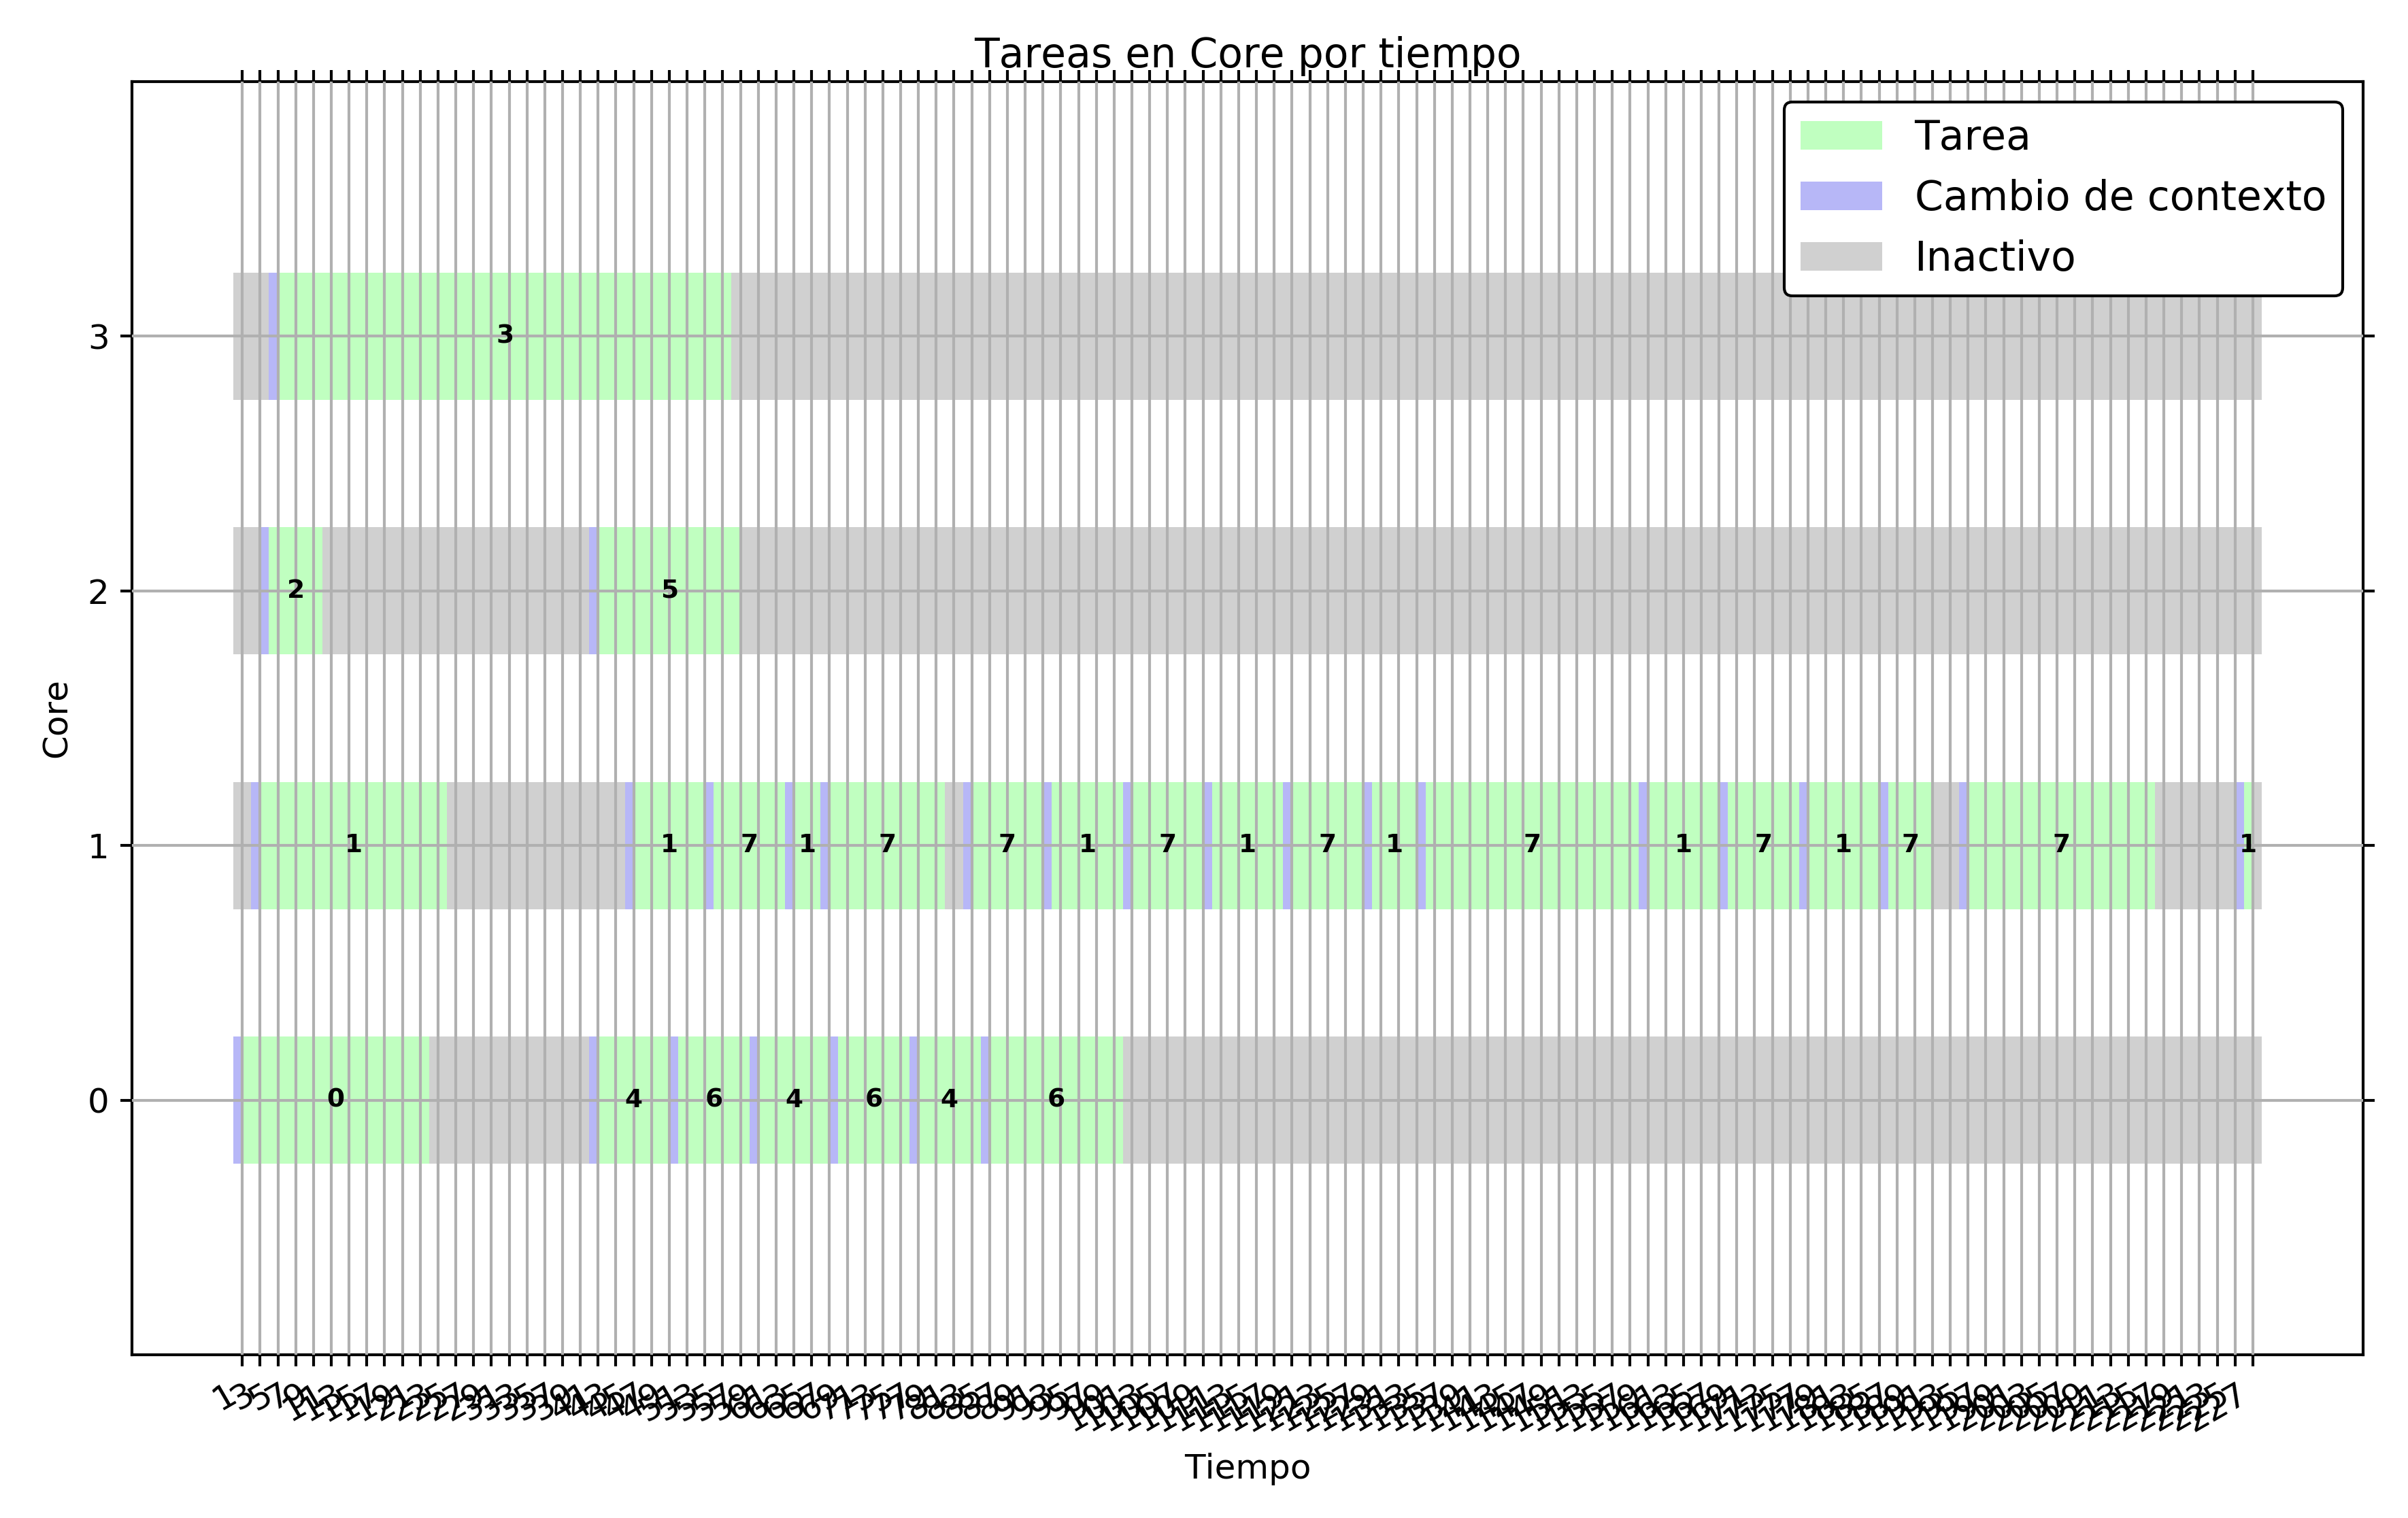
\includegraphics[width=1\textwidth]{images/ej8/lote2_cores.png}
  \label{fig: lote8_2_cores}
  \caption{Diagrama de uso de nucleos del lote 2.}
\end{figure}

\par En la figura \ref{fig: lote8_2_cores} podemos ver que los nucleos 0, 2 y 3 se liberan rápidamente mientras que el 1 continúa ejecutando por largo tiempo. Esto se debe a que quedan dos procesos pesados (el 1 y el 7) corriendo en el nucleo 1 y el scheduler no migra alguno de estos a otro nucleo.

\begin{figure}[h]
  \centering
    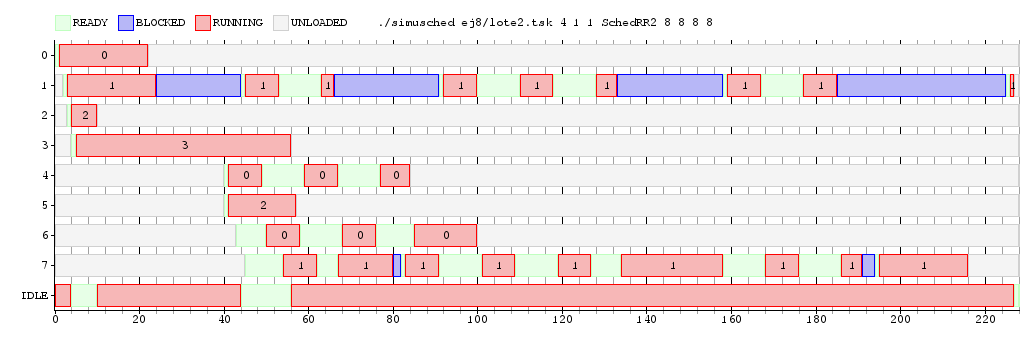
\includegraphics[width=1\textwidth]{images/ej8/lote2_sched.png}
  \label{fig: lote8_2_sched}
  \caption{Diagrama de procesos del lote 2.}
\end{figure}

\par En la figura \ref{fig: lote8_2_sched} podemos ver los procesos y sus estados con el paso del tiempo. Aquí también podemos notar que los procesos 1 y 7 son los que utilizan mas tiempo el CPU (y antes vimos que justo caen en el mismo nucleo). \\\\

\par Analicemos el rendimiento del scheduler:
\begin{itemize}
	\item \textbf{Fairness:} \\
	Se trata de un scheduler Round-Robin y podemos ver que distribuye un quantum a cada uno de la cola en órden.
	\item \textbf{Tiempo de respuesta:}\\
	Promedio: $\frac{1 + 1 + 1 + 1 + 1 + 1 + 7 + 9}{8} = 2,75$
	\item \textbf{Throughput:}\\
	Promedio: $\frac{1 + 1 + 1 + 1 + 1 + 1 + 1 + 1}{228} = 0,035$
	\item \textbf{Turnaround:}\\
	Promedio: $\frac{(22 - 0) + (227 - 2) + (10 - 3) + (56 - 4) + (84 - 40) + (57 - 40) + (100 - 43) + (216 - 45)}{8} = 74,375$ \\
	El número no parece ser favorable porque la mayoría de los procesos tienen una longitud corta. Pero el proceso mas largo tiene longitud aproximada 90, por lo que no parece tan alejado del valor obtenido.
	\item \textbf{Waiting time:}\\
	Promedio: $\frac{1 + (1 + 1 + 10 + 10 + 10 + 1 + 10 + 1) + 1 + 1 + (1 + 10 + 10) + 1 + (7 + 10 + 9) + (9 + 5 + 1 + 10 + 10 + 7 + 10 + 10 + 1)}{8} = 19,75$
\end{itemize}

\par La diferencia mas grande se nota en el valor de Throughput. El ejemplo del caso beneficioso al scheduler nos daba un valor de $0,1829$, mientras que el ejemplo del caso no beneficioso al scheduler nos daba un valor de $0,035$ (5 veces menor). Esto se debe a lo que comentábamos de la migración de procesos entre nucleos. En general se trata de evitar, pero para casos como el que tomamos como ejemplo no beneficioso puede ser útil y ayudar a aliviar un nucleo.
\par En la figura \ref{fig: lote8_2_cores} se ve claramente el uso de un nucleo mientras que el resto se encuentran liberados y podrían ser utilizados para alivianar la carga sobre este.